\section{Structures Management}

Selecting "Structures" from the navigation drawer displays the Structures management view. This page presents a tabular inventory of layout buildings and trackside structures, summarizing attributes such as Title, Use, Owner, layout Location, Year Built, and Action controls. Figure \ref{fig:structures} shows the main Structures table page.

\begin{figure}[H]
    \centering
    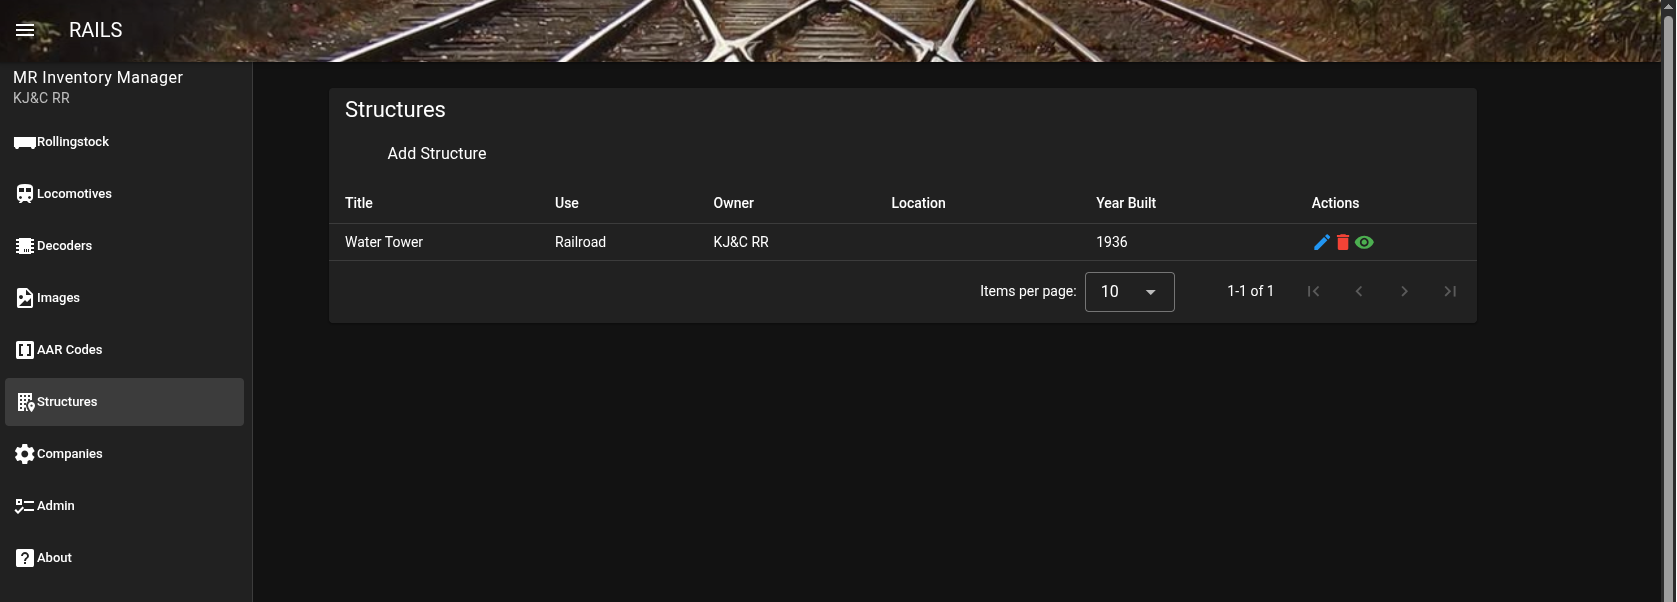
\includegraphics[width=0.85\textwidth]{./images/structures.png}
    \caption{Structures Page}
    \label{fig:structures}
\end{figure}

\subsection{Viewing Structure Details}

Clicking the green eye icon in the Actions column opens a detail view modal. This dialog presents recorded attributes alongside an embedded photo preview of the modeled structure. Figure \ref{fig:structures-view} displays the structure inspection dialog.

\begin{figure}[H]
    \centering
    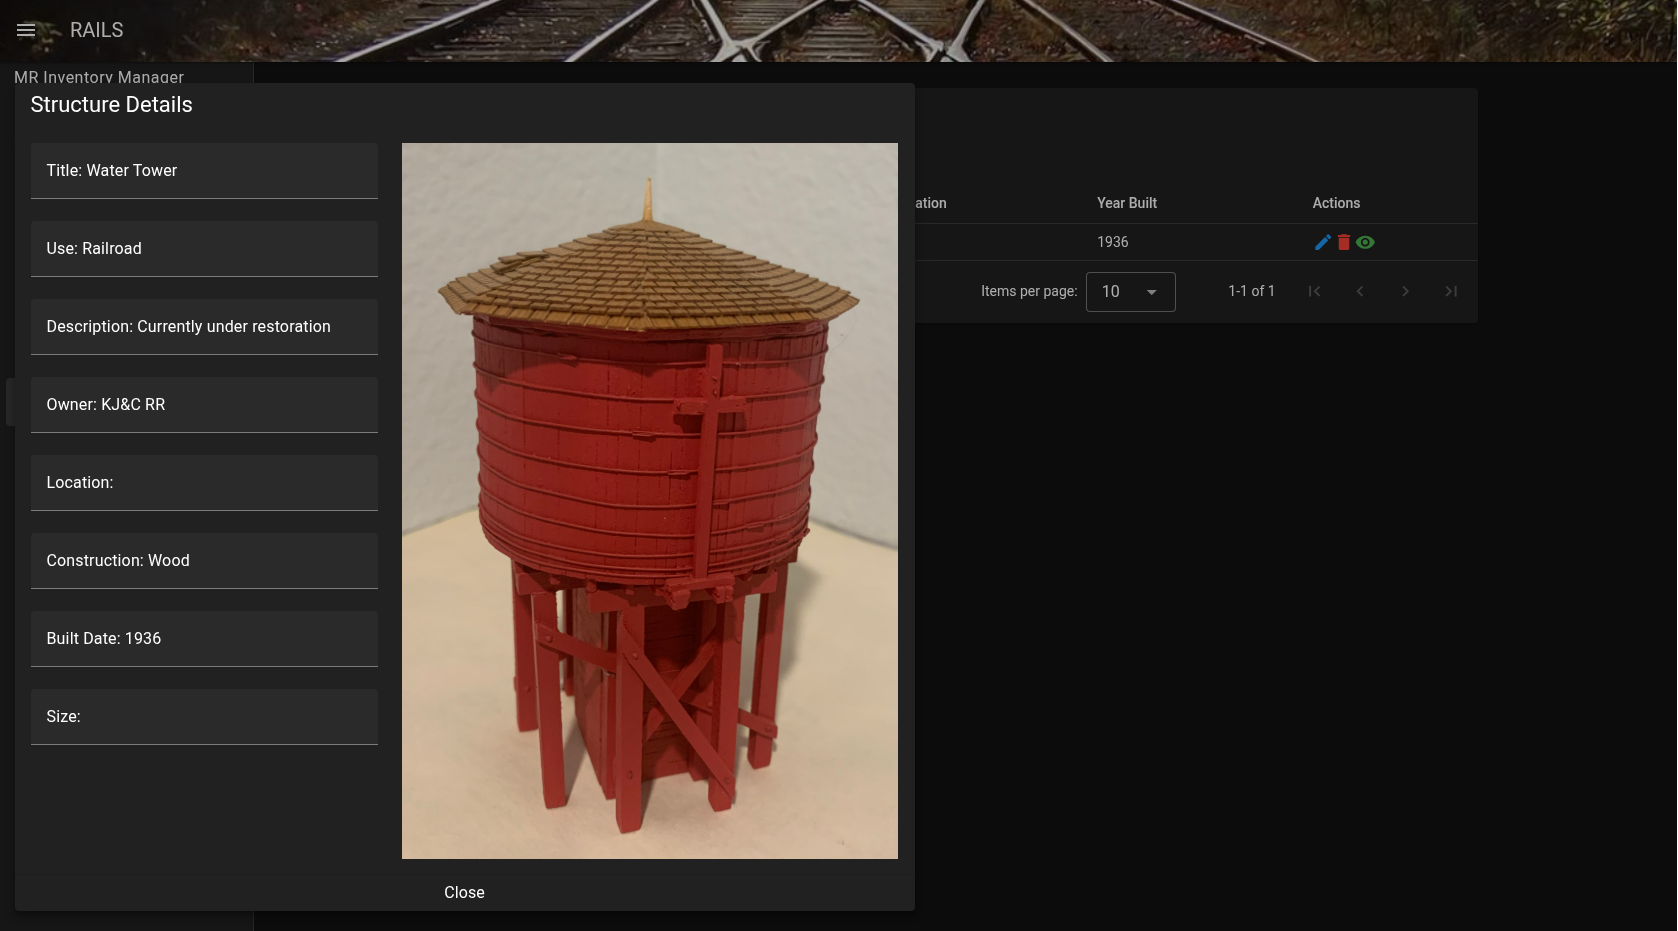
\includegraphics[width=0.85\textwidth]{./images/structures-view.png}
    \caption{View Structure Details}
    \label{fig:structures-view}
\end{figure}

\subsection{Adding a New Structure}

Clicking the "Add Structure" button above the table opens a modal dialog for adding a new building or facility to the database. The form includes comprehensive fields for general metadata (Title, Use, Owner, Location, Construction, Built Date, Size, Image) and operational parameters (Industrial classification, Type, Raw Materials, Capacities, Production Rates, Priority, AAR Codes In/Out, Load/Unload Durations, Siding Capacity, and Notes). Figure \ref{fig:structures-new} illustrates the structure creation modal.

\begin{figure}[H]
    \centering
    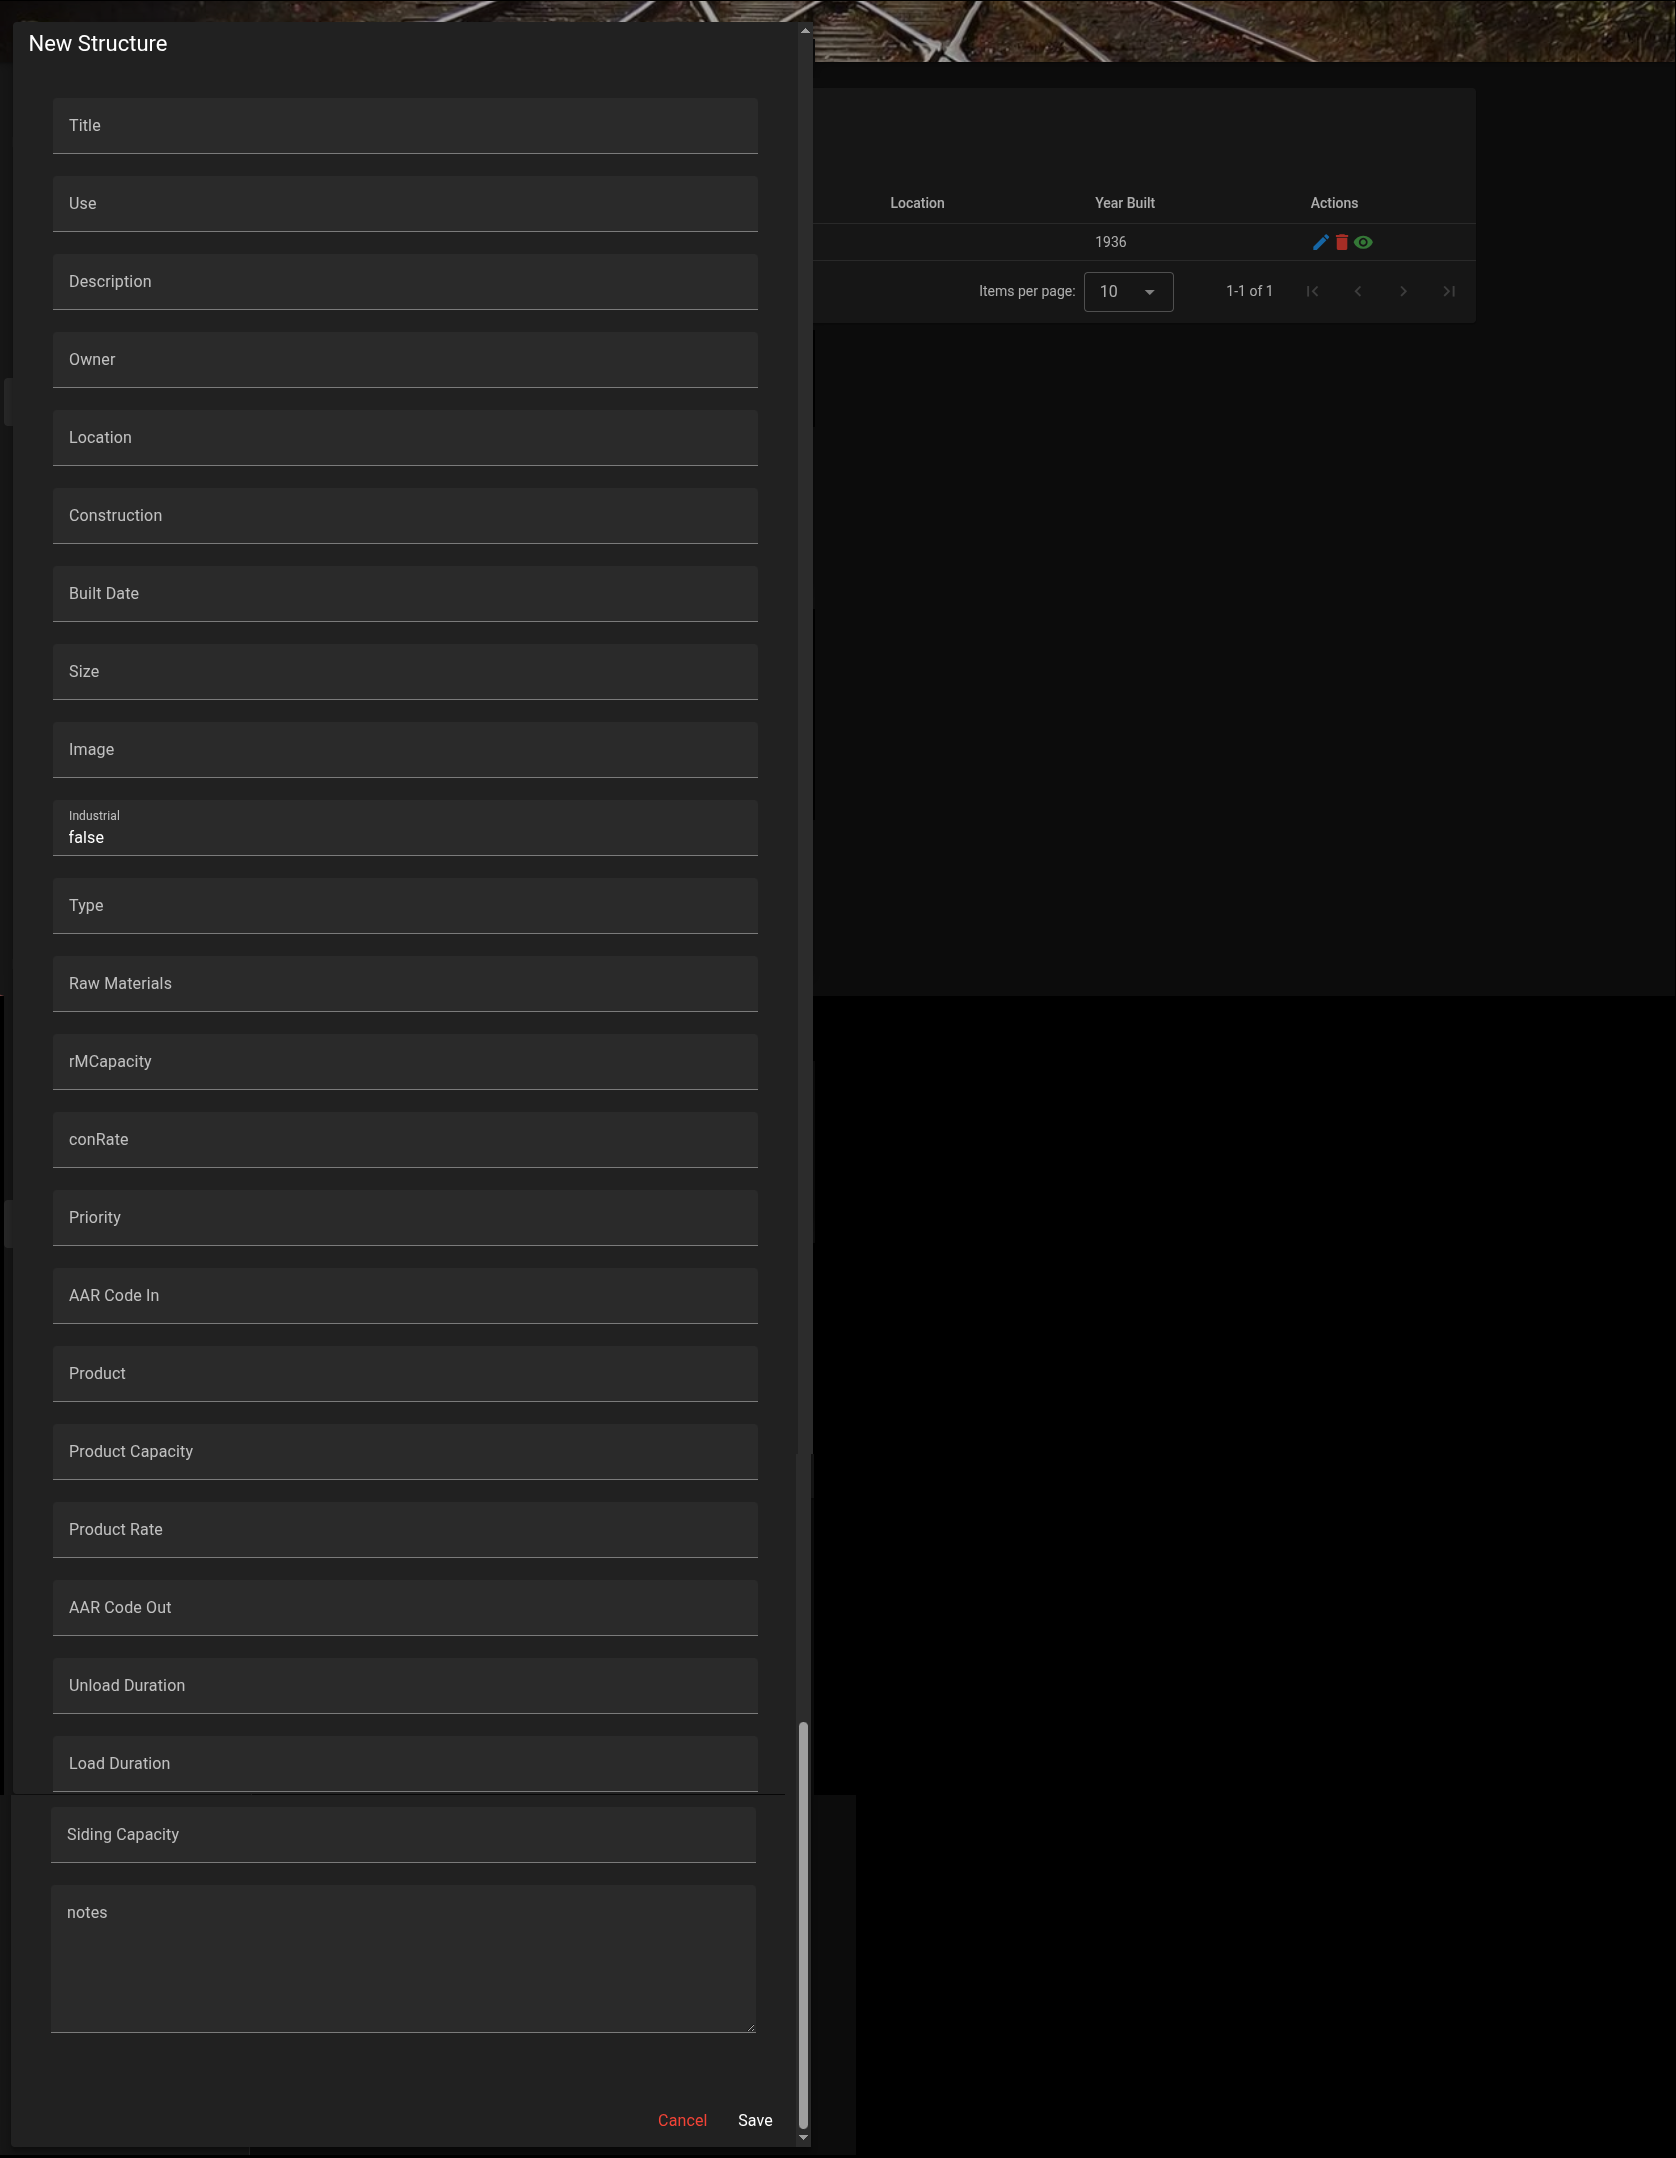
\includegraphics[width=0.85\textwidth]{./images/structures-new.png}
    \caption{Add Structure Dialog}
    \label{fig:structures-new}
\end{figure}

\subsection{Editing Structure Records}

To update an existing entry, click the blue pencil icon under the Actions column. This opens the structure form populated with current records, allowing edits to physical attributes, image references, or industrial operational data. Figure \ref{fig:structures-edit} shows the edit structure dialog.

\begin{figure}[H]
    \centering
    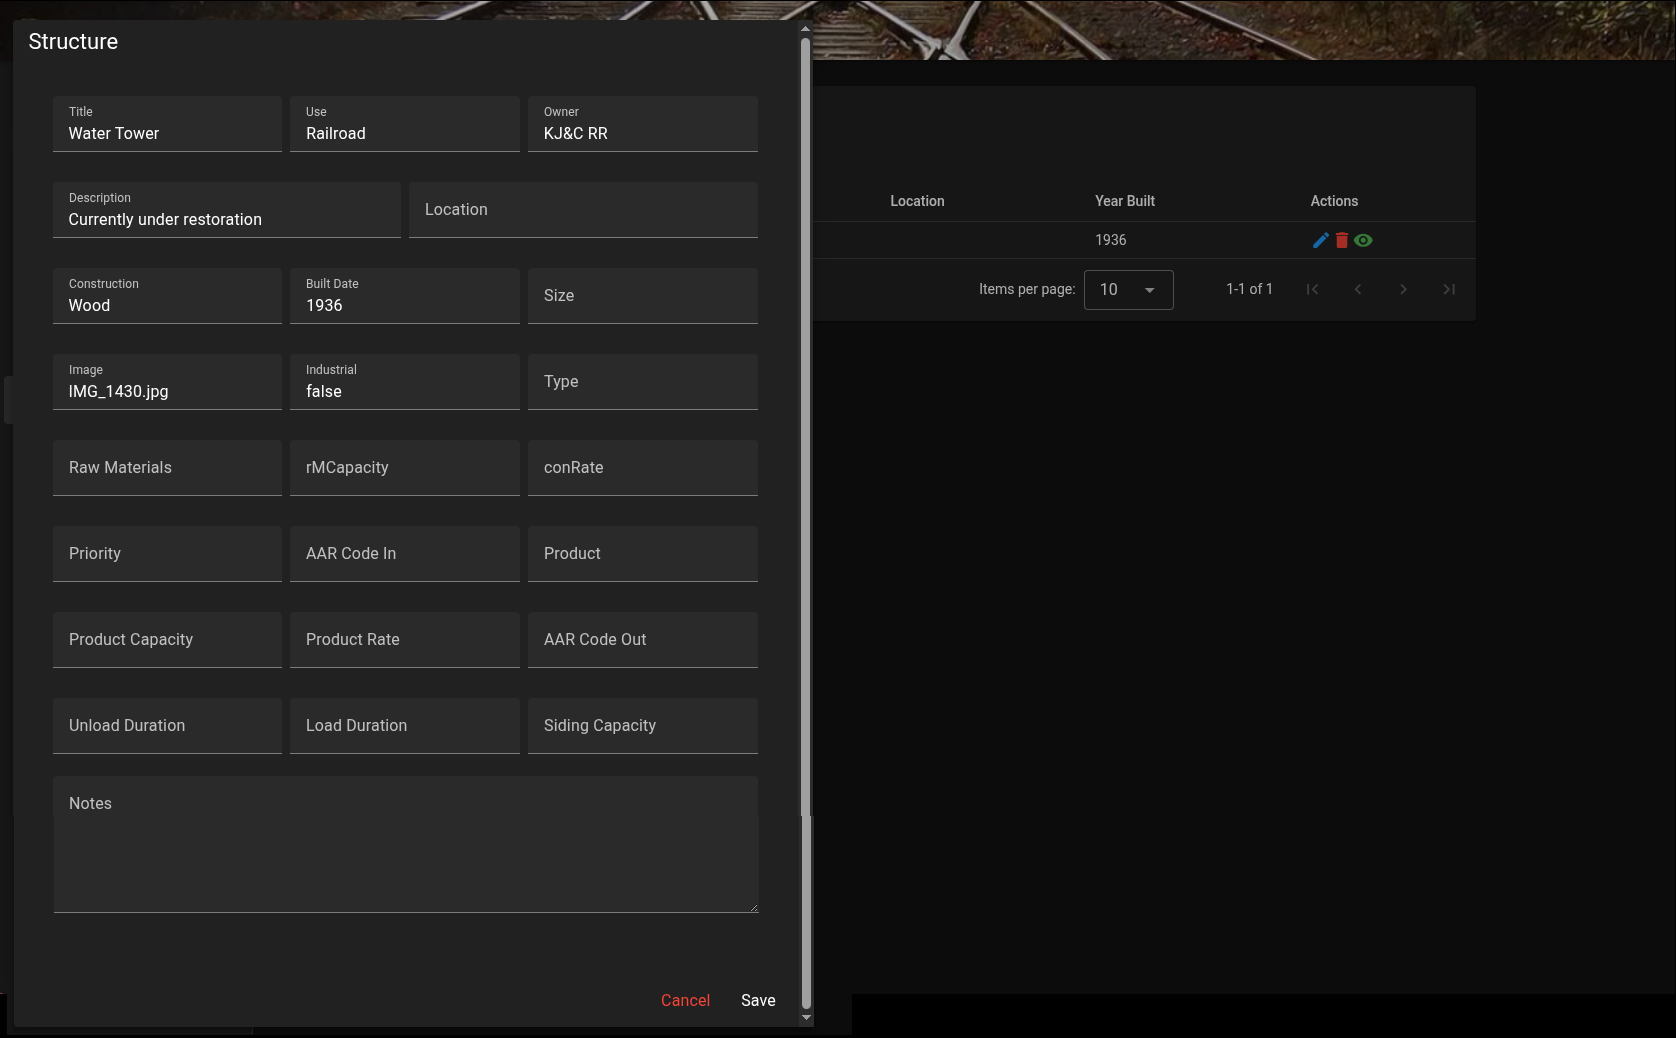
\includegraphics[width=0.85\textwidth]{./images/structures-edit.png}
    \caption{Edit Structure}
    \label{fig:structures-edit}
\end{figure}

\subsection{Deleting Structure Records}

To remove a structure entry from the inventory, click the red trash bin icon in the Actions column. A confirmation prompt appears requiring verification before the record is deleted from the system database. Figure \ref{fig:structures-delete} illustrates the deletion modal dialog.

\begin{figure}[H]
    \centering
    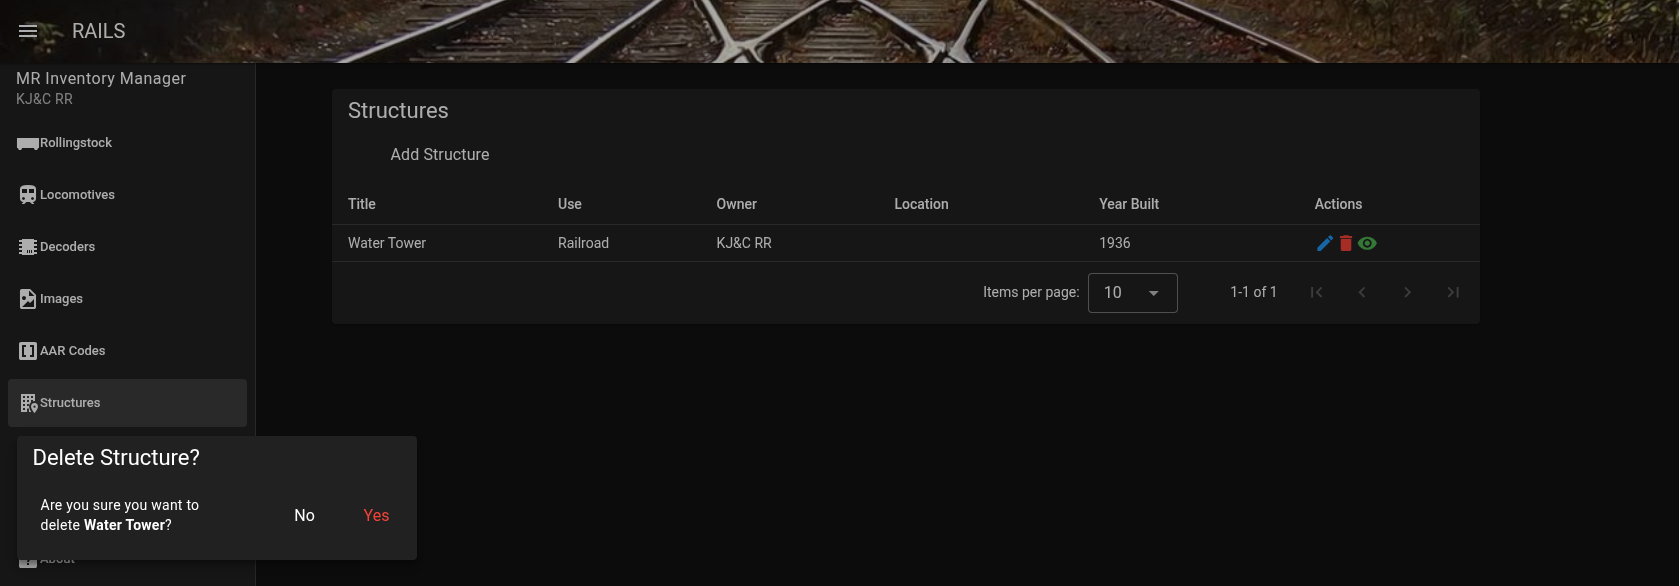
\includegraphics[width=0.85\textwidth]{./images/structures-delete.png}
    \caption{Delete Structure Confirmation}
    \label{fig:structures-delete}
\end{figure}
